\PassOptionsToPackage{xetex}{xcolor}
\PassOptionsToPackage{xetex}{graphicx}
\documentclass[a4paper,landscape,headrule,footrule,xetex]{foils}

\input{headx.tex}
\usepackage{tikz}
\usepackage{colortbl}
\definecolor{Gray}{gray}{0.9}

\usepackage{newunicodechar}

\newcommand\Warning{%
 \makebox[1.4em][c]{%
 \makebox[0pt][c]{\raisebox{.1em}{\small!}}%
 \makebox[0pt][c]{\color{red}\Large$\bigtriangleup$}}}%

\newunicodechar{⚠}{\Warning}

\begin{document}
\header{Lecture 4}{Quantification, Truth and Sentiment}{}
\maketitle

%\include{schedule}


\myslide{Overview}

\begin{itemize}
%\item Revision of sentence meaning and compositionality
\item Truth and Logic
\item Quantification and Negation
\item Sentiment and Connotation
\item Presupposition
\end{itemize}



\myslide{Motivation}

\begin{itemize}
\item Logic is expressed in sometimes unexpected ways in natural
  language, we will look at some of these examples (Quantification and Negation)
\item We use language to reason, as we can see in the Holmes's stories
  \begin{itemize}
  \item Sherlock looks at the evidence
  \item and forms conclusions
  \end{itemize}
  We will look at how we can do this (Truth and Logic)
\item Finally, language is expressive because of the
  color: the way Doyle paints different characters as good or evil
  (Sentiment and Connotation)
\end{itemize}


% \section{Revision}

% \myslide{Meaning is built up Compositionally}

% \begin{itemize}
% \item \txx{Compositional Semantics}: the meaning of the whole depends (only)
%   on the meanings of the parts and the method of combination.
% \item The hearer/reader's \txx{interpretation} brings in much more
%   \begin{itemize}
%   \item we bring in our existing knowledge
%   \item we make inferences
%   \end{itemize}
% \item These inferences are based on (or constrained by) the semantics
% \item Intersective modification constrains the denotation
% \end{itemize}

% \myslide{Sentences describe situations}

% \begin{itemize}
% \item Semantic Roles describe interactions of the participants 
%   \\ and possibly the location, time, manner, reason and so forth
% \item Roles are constrained by the verb (or adjective, \ldots) but can
%   also be used to generalize
% \item Verbs can appear with different roles filling different
%   syntactic positions (alternations).
%   \\ \eng{I broke the window} vs \eng{The window broke}
% \end{itemize}

% \myslide{Tense, Aspect and Modality}

% \begin{itemize}
% \item We can talk about when things occurred (tense)
%   \begin{exe}
%     \ex \eng{I did it.}
%   \end{exe}
% \item Whether they are still ongoing (aspect)
%   \begin{exe}
%     \ex \eng{I am doing it.}
%   \end{exe}
% \item Whether we think something is true or should be (modality)
%   \begin{exe}
%     \ex \eng{I should probably go}
%     \ex \eng{I must have that}
%   \end{exe}
% \end{itemize}

% \myslide{Close Reading}
% \begin{itemize}
% \item Reading (and often re-reading) a text to uncover multiple
%   aspects of meaning that lead you to understand a text better
% \item This involves looking at what the text actually says, as well as
%   the inferences you make from reading it
% \item After a close reading you should be able to support your
%   conclusions with specific examples from the text
% \item You can consider many aspects of the text, we focus on word
%   choice
% \item We do this in Projects 1 and 2.
% \end{itemize}

\section{Reasoning}
\begin{quote}  
\textsc{Sherlock:} \eng{``You will not apply my precept," he said, shaking his head. "How often have I said to you that when you have eliminated the impossible, whatever remains, however improbable, must be the truth? We know that he did not come through the door, the window, or the chimney. We also know that he could not have been concealed in the room, as there is no concealment possible. When, then, did he come?''}

\begin{flushright}
   The Sign of the Four (\sh{SIGN}) 
\end{flushright}
\end{quote}



\myslide{Three Kinds of Reasoning}
\begin{itemize}
\item \txx{Deductive Reasoning} allows you to start from general
  premises or categories, then to prove a specific conclusion (100\%).
\item \txx{Inductive Reasoning} is reasoning in which the premises
  give evidence for the degree of truth of the conclusion (probably).
\\ \eng{We balance probabilities and choose the most likely. It is the scientific use of the imagination.} (\sh{HOUN})
\item \txx{Abductive Reasoning} goes from observation to
  hypothesis.  The goal is to find the theory which best accounts for
  the observation, ideally seeking to find the simplest and most
  likely explanation.
\end{itemize}

Holmesian deduction is abductive reasoning:
\begin{itemize} \addtolength{\itemsep}{-1ex}
\item come up with explanations
\item eliminate wrong ones (using deductive reasoning)
\item the remaining one is the best explanation
\end{itemize}




\myslide{Logic (Deductive Reasoning)}

\begin{itemize}
\item Classical logic is an attempt to find valid principles of argument and inference.
\\[2ex]
\begin{tabular}{llr}
  $a$ & Humans are mortal & \txx{premise} \\
  $b$ & Socrates is human & \txx{premise}\\ \hline
  $c$ & Socrates is mortal & \txx{conclusion}
\end{tabular}
\item Can we go from $a$ and $b$ to $c$? \hfill {\large Yes}
\item Truth is \txx{empirical}: The premises need to correspond with
  the facts of the world
  \begin{itemize}
  \item Sentences have \txx{truth values} (true, false or unknown)
  \item The state of the world that makes a sentence true or false are its \txx{truth conditions}
  \end{itemize}
\end{itemize}


\myslide{Logical Connectives}
\MyLogo{It isn't just saying \textit{no it isnt't}}
\begin{itemize}
\item \txx{and} ($p \wedge q$: conjunction) \hfill \ces{a} \\
  — both must be true
\item \txx{or} ($p \vee q$: disjunction, inclusive or) \hfill \ces{nebo} \\
  — at least one must be true
\item \txx{xor} ($p \oplus q$: exclusive or, either or) \hfill \ces{exkluzivní nebo/buď anebo} \\
  — exactly one must be true
\item \txx{if} ($p \rightarrow q$: implication) \hfill \ces{jestliže} \\
  — if $p$ is true, then $q$ must be true
\item \txx{iff} ($p \equiv q$: if and only if) 
  ($(p \rightarrow q) \wedge (q \rightarrow p)$) \hfill \ces{právě tehdy, když} \\
  —  both must be true or both false
\item \txx{not} ($\neg p$: negation) \hfill \ces{ne} \\
  — not $p$ is true when $p$ is false (and false when $p$ is true)
% % If it doesn’t rain, p = F, the conditional claim cannot be
% % invalidated by whatever is done. (q= T or q =F). p is a
% % sufficient but not necessary condition for q. Some other
% % factor might want to cause me to go to the movies!
% % But not all if.. then…constructions work like that. What are
% % some counterexamples that you can think of? If she is smart,
% % then I would win the Nobel prize (counterfactuals)
\end{itemize}


\myslide{Truth Tables}
\MyLogo{\textit{Yes it is}}
\begin{center}
  \begin{tabular}{|c|c|c|c|c|c|c|c|}
    \hline
    $p$ & $q$ & $p \rightarrow q$ & $p \wedge q$ & $p \vee q$ 
    & $p \oplus q$ & $p \equiv q$ & $\neg p$\\
    \hline
    &   & if & and & or &  XOR & iff & not  \\
    \hline
    T & T & T & T & T & F & T & F \\ 
    T & F & F & F & T & T & F & F \\  
    F & T & T & F & T & T & F & T\\ 
    F & F & T & F & F & F & T & T\\ \hline
%    \hline
  \end{tabular}

  
\end{center}
  \begin{itemize}
  \item Words themselves often carry more implications
    \\ \eng{I did A and B} often implies \eng{I did A first}
  \item There are many ways of saying the operations
\item \txx{entailment} ($\vdash$: logical consequence, $\therefore$)) something
  logically follows from the preceding statements
\end{itemize}
\begin{quote}
  An \txx{argument} is a connected series of statements attempting to
  establish a proposition.
\end{quote}




\myslide{Logical Connectives as Graphs ($p$ and $\neg p$)}
\MyLogo{\textit{No it isnt't}}
 
\begin{tabular}{cc}
$p$   & $\neg p$ ``not'' \\[2ex] 
\scalebox{2}{
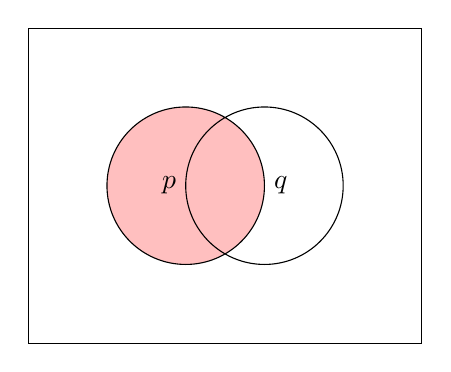
\begin{tikzpicture}
\filldraw[fill=white] (-2,-2) rectangle (3,2);
\scope % A \cap B
%\clip (0,0) circle (1);
\fill[pink] (0,0) circle (1);
\endscope
% outline
\draw (0,0) circle (1) node [text=black,left] {$p$}
      (1,0) circle (1) node [text=black,right] {$q$};
\end{tikzpicture}} &
\scalebox{2}{
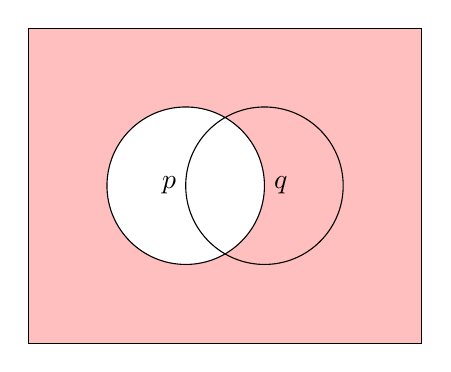
\begin{tikzpicture}
\filldraw[fill=pink] (-2,-2) rectangle (3,2);
\scope % A \vee B
%\clip (0,0) circle (1);
%\fill[pink] (1,0) circle (1);
\fill[white] (0,0) circle (1);
\endscope
\draw (0,0) circle (1) node [text=black,left] {$p$}
      (1,0) circle (1) node [text=black,right] {$q$};
% outline
\end{tikzpicture}}

\end{tabular}

\myslide{Logical Connectives as Graphs ($p \wedge q$ and   $p \vee q$)}
\MyLogo{\textit{Yes it is}}

\begin{tabular}{cc}
$p \wedge q$ ``and''  & $p \vee q$ ``or'' \\[2ex]  
\scalebox{2}{
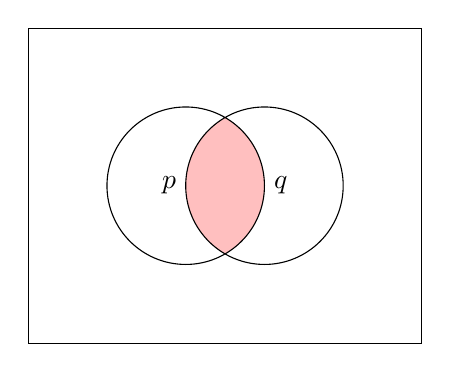
\begin{tikzpicture}
\filldraw[fill=white] (-2,-2) rectangle (3,2);
\scope % A \cap B
\clip (0,0) circle (1);
\fill[pink] (1,0) circle (1);
\endscope
% outline
\draw (0,0) circle (1) node [text=black,left] {$p$}
      (1,0) circle (1) node [text=black,right] {$q$};
\end{tikzpicture}} &
\scalebox{2}{
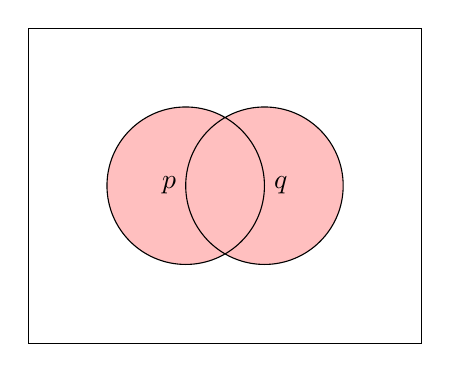
\begin{tikzpicture}
\filldraw[fill=white] (-2,-2) rectangle (3,2);
\scope % A \vee B
%\clip (0,0) circle (1);
\fill[pink] (1,0) circle (1);
\fill[pink] (0,0) circle (1);
\endscope
% outline
\draw (0,0) circle (1) node [text=black,left] {$p$}
      (1,0) circle (1) node [text=black,right] {$q$};
\end{tikzpicture}}
\end{tabular}


\myslide{Logical Connectives as Graphs ($p \oplus q$ and   $p \rightarrow q$)}
\MyLogo{\textit{No it isnt't}}

\begin{tabular}{cc}
$p \oplus q$ ``exclusive or''  & $p \rightarrow q$ ``if'' \\[2ex] 
\scalebox{2}{
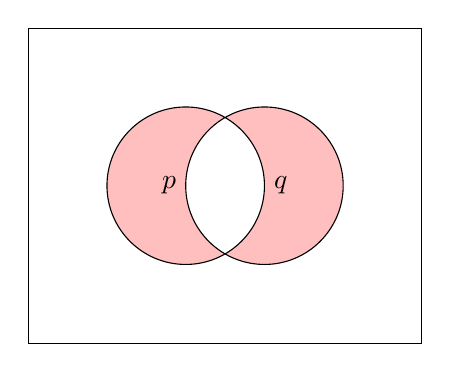
\begin{tikzpicture}
\filldraw[fill=white] (-2,-2) rectangle (3,2);
\fill[pink] (1,0) circle (1);
\fill[pink] (0,0) circle (1);
\scope % A \cap B
\clip (0,0) circle (1);
\fill[white] (1,0) circle (1);
\endscope
% outline
\draw (0,0) circle (1) node [text=black,left] {$p$}
      (1,0) circle (1) node [text=black,right] {$q$};
\end{tikzpicture}} &
\scalebox{2}{
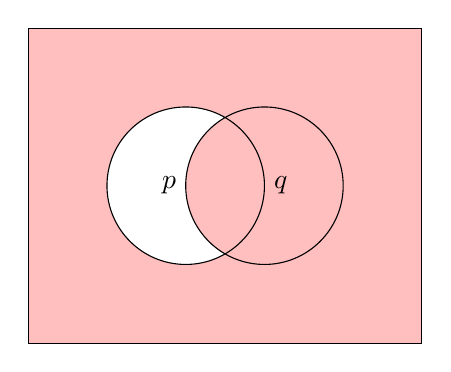
\begin{tikzpicture}
\filldraw[fill=pink] (-2,-2) rectangle (3,2);
\scope % A \vee B
%\clip (0,0) circle (1);
\fill[white] (0,0) circle (1);
\fill[pink] (1,0) circle (1);
\endscope
% outline
\draw (0,0) circle (1) node [text=black,left] {$p$}
      (1,0) circle (1) node [text=black,right] {$q$};
\end{tikzpicture}}
\end{tabular}





\myslide{Semantic Relations as Graphs ($p \subset q$ and $p \sim q$)}
\MyLogo{\textit{Yes it is}}

\begin{tabular}{cc}
$p \subset q$ \iz{hypernym}  & $p \sim q$ \iz{synonym} \\[2ex] 
\scalebox{2}{
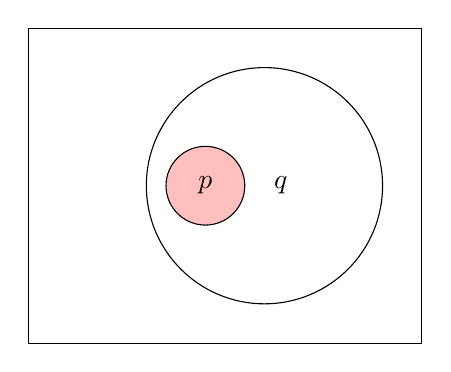
\begin{tikzpicture}
\filldraw[fill=white] (-2,-2) rectangle (3,2);
\scope % A \vee B
%\clip (0,0) circle (1);
\fill[pink] (0.25,0) circle (0.5);
%\fill[white] (0,0) circle (1);
\endscope
\draw (0.25,0) circle (0.5) node [text=black] {$p$}
      (1,0) circle (1.5) node [text=black,right] {$q$};
% outline
\end{tikzpicture}}
&
\scalebox{2}{
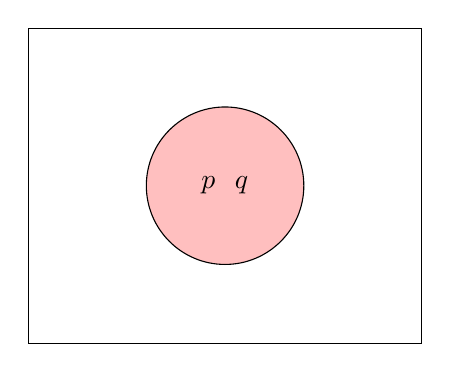
\begin{tikzpicture}
\filldraw[fill=white] (-2,-2) rectangle (3,2);
\scope % A \vee B
%\clip (0,0) circle (1);
%\fill[pink] (1,0) circle (1);
\fill[pink] (0.5,0) circle (1);
\endscope
\draw (0.5,0) circle (1) node [text=black,left] {$p$}
      (0.5,0) circle (1) node [text=black,right] {$q$};
% outline
\end{tikzpicture}}

\end{tabular}


%\section{Deductive Reasoning}

\myslide{Modus ponens}
\MyLogo{\textit{No it isnt't}}
\begin{center}
  \begin{tabular}{llcl}
    $a$ & All humans are mortal & $p  \rightarrow q$ & 
    \small if someone is human then they are mortal\\
    $b$ & Socrates is human & $p$ \\ \hline
    $c$ & Therefore, Socrates is mortal & $q$
  \end{tabular}


  \begin{tabular}{|c|c|c|c|c|c|c|}
    \hline
    $p$ & $q$ & $p \rightarrow q$  \\
    \hline
    \rowcolor{Gray}
    \textbf{T} & T & \textbf{T}  \\ 
    \textbf{T} & F & F  \\ 
    F & T & \textbf{T}  \\ 
    F & F & \textbf{T}  \\ 
    \hline
  \end{tabular}
\end{center}
\begin{itemize}
\item  The way that affirms by affirming (Latin)
\item $p \rightarrow q, p \vdash q$    (if $p$ then $q$,  and $p$ implies $q$)
\item \txx{material implication}  (Not quite the same as English \lex{if})
\end{itemize}

\myslide{Modus tollens}
\MyLogo{\textit{Yes it is}}
\begin{center}
  \begin{tabular}{llc}
    $a$ & If something is human then it is mortal & $p  \rightarrow q$\\
    $b$ & Zeus is not mortal  & $\neg q$ \\ \hline
    $c$ & Zeus is not human   & $\neg p$
  \end{tabular}

  \begin{tabular}{|c|c|c|c|c|c|c|}
    \hline
    $p$ & $q$ & $p \rightarrow q$  \\
    \hline
    T & T & \textbf{T}  \\ 
    T & \textbf{F} & F  \\ 
    F & T & \textbf{T}  \\ 
    \rowcolor{Gray}
    F & \textbf{F} & \textbf{T}  \\ 
    \hline
  \end{tabular}
\end{center}
\begin{itemize}
\item  The way that negates by negating (Latin)
\item $p \rightarrow q, \neg q \vdash \neg p$   (if $p$ then $q$, and not $q$  implies not $p$)
\end{itemize}

\myslide{Other types of syllogisms}
\MyLogo{\textit{No it isnt't}}

\begin{itemize}
\item \txx{Hypothetical syllogism}
\\[2ex]
 \begin{tabular}{ll}
    $a$ & If something is human then it is mortal \\
    $b$ & If something is mortal then it dies \\ \hline
    $c$ & If something is human then it dies
  \end{tabular}
\\ $p \rightarrow q, q \rightarrow r \vdash p \rightarrow r$

\item \txx{Disjunctive syllogism}
\\ (modus tollendo ponens: affirm by denying)
\\[2ex]
 \begin{tabular}{ll}
    $p$ & Either a human is mortal or a human is immortal \\
    $q$ & A human is not immortal \\ \hline
    $r$ & A human is mortal
  \end{tabular}
\\ $p \oplus q, \neg p \vdash q$
\end{itemize}

These are all ways of proving something is true.


\myslide{Bad Arguments}
\MyLogo{And many, many more}
\begin{itemize}
\item Formal (can be disproved with truth tables)
  \begin{itemize}
  \item \txx{Affirming the consequent}: $p \rightarrow q, q \vdash p$
    \\ \eng{professors talk too much}, \eng{you talk too much} $\vdash$ \eng{you are a professor}
  \end{itemize}
\item Informal
  \begin{itemize}
  \item \txx{Equivocation}:  The sign said \eng{fine for parking here}, and since it was fine, I parked there. 
  \item \txx{No True Scotsman}: X doesn't do Y; $a$ is an X and does Y; $a$ is not a true X
  \item \txx{Slippery Slope}: We mustn't allow text abbreviations or students will not be able to write normal text.
  \item \txx{False Dilemma}: You are with us or against us [or possibly don't care]
  \item \txx{Guilt by Association}: Hitler was a vegetarian  $\vdash$ vegetarianism is bad
  \end{itemize}
  \begin{center}
     ⚠ -- a bad argument doesn't mean the conclusion is wrong\\
    just that the argument doesn't prove it, \ldots
  \end{center}

\end{itemize}


\myslide{Arguments in Sherlock Holmes}

\begin{itemize}
\item Most of the deduction in Sherlock Holmes depends on having a
  very restricted set of possibilities
  \begin{itemize}
  \item partly a literary trick: the author controls the world they write about
    \begin{itemize}
    \item Holmes is very lucky in his choice of theories
    \end{itemize}
  \item partly a reflection of the stratification of Victorian society
    \begin{itemize}
    \item there are many hypotheses based on stereotypes
    \item \textsc{Sherlock:} \eng{There is no vehicle save a dog-cart which throws up mud in that way, and then only when you sit on the left-hand side of the driver.} 
    \end{itemize}
  \end{itemize}
\end{itemize}


\myslide{Arguments in Sherlock Holmes: Jabez}

\begin{itemize}
\item \eng{Beyond the obvious facts that} \hfill (conclusions)
  \begin{itemize}
  \item  \eng{he has at some time done manual labour}, 
    \\ his right hand is stronger than his left
  % \item  he takes snuff, 

  \item  \eng{he is a Freemason}, 
    \\ an arc and compass breastpin
  \item  \eng{he has been in China}
    \\ pink tattoo and coin
  \item  \eng{he has done a considerable amount of writing lately}
    \\ smooth patch on right cuff and left elbow
  \end{itemize}
  \item[?] Can you come up with alternative explanations?\task
\end{itemize}







\section{Quantification and Negation}

\myslide{Shades of meaning}
\begin{itemize}
\item We can restrict the scope of statements with quantifiers
\item We can change the polarity of statements using negation
\item These interact with each other in interesting ways
\item These interact with language in interesting ways
\end{itemize}

\myslide{Simple Statements in Predicate Logic}
\MyLogo{Ignore tense for the moment}

\begin{itemize}
\item Consider simple sentences
  \begin{itemize}
  \item Represent the \txx{predicates} by a capital letter
    \\ these can be $n$-ary
  \item Represent the \txx{individual constants} by lower case letters
  \item Represent \txx{variables} by lower case letters (x,y,z)
  \end{itemize}
  \begin{exe}
    \ex \eng{Bobbie is asleep}: A(b)
    \ex \eng{Freddie drinks}: D(f)
    \ex \eng{Freddie drinks beer}: D(f,b)
    \ex \eng{Freddie prefers beer to whiskey}: P(f,b,w)
    \ex \eng{Someone is asleep}: A(x) \hfill (A(x) $\wedge$ P(x)) 
  \end{exe}
\end{itemize}

\myslide{Complex Statements in Predicate Logic}
\MyLogo{Ignore tense for the moment}

\begin{itemize}
\item Join simple sentences with logical connectives
\\ treat relative clauses as \txx{and}
  \begin{exe}
    \ex \eng{Bobbie who is asleep writhes}: A(b) $\wedge$ W(b)
    \ex \eng{Bobbie is asleep and Freddie drinks}: A(b) $\wedge$ D(f)
    \ex \eng{Freddie drinks and sleeps}: D(f) $\wedge$ S(f)
    \ex \eng{Freddie doesn't drink beer}: $\neg$ D(f,b)
    \ex \eng{If Freddie drinks whiskey Bobbie sleeps}: D(f,w) \into S(b)
%    \ex \eng{x is asleep}: A(x)
  \end{exe}
\item If you run out of letters, use two, keep them unique in the
  world you are modeling
 \begin{exe}
    \ex \eng{Bobbie who is asleep snores}: A(b) $\wedge$ Sn(b)
  \end{exe}
\end{itemize}


\myslide{Quantifiers in Predicate Logic}
\MyLogo{Keep ignoring tense, we are also ignoring number;
assume a simple world of predicates and individuals (constant and variable)}

\begin{itemize}\addtolength{\itemsep}{-1ex}
  \item Quantifiers bind variables and scope over predications
    \begin{itemize}
    \item \txx{Universal Quantifier} ($\forall$: \eng{each, every, all})
      \hfill \ces{univerzální kvantifikátor} \\
      --- true for every element \hfill \ces{for all/pro všechna}
    \item \txx{Existential Quantifier} ($\exists$: \eng{some, a})
      \hfill \ces{existenciální kvantifikátor} \\
      --- true for at least one element \hfill \ces{exists/existuje} 
    \begin{exe}
      \ex \eng{All students learn logic}: $\forall$x (S(x)  $\into$ L(x,l))
      \ex \eng{A student learns logic}: $\exists$x (S(x)  $\wedge$ L(x,l))
      \ex \eng{Some students learn logic}: $\exists$x (S(x)  $\wedge$ L(x,l))
      \ex\label{me} \eng{No students learn logic}: $\neg\exists$x (S(x)  $\wedge$ L(x,l))
      \ex \eng{All students don't learn logic}: $\forall$x (S(x)  $\into$ $\neg$L(x,l))
      \\ logically equivalent to (\ref{me})
    \end{exe}
  \item $\forall$ must check each one (so $\into$)
  \item $\exists$ is falsified by one counter example  (so $\wedge$)
    \end{itemize}

  \item All variables must be bound \\
    If there is an x, y, z it must have a $\forall$ or $\exists$
\end{itemize}

\myslide{Why Translate to Predicate Logic}
\MyLogo{Often people omit the P(x), P(y)}

\begin{itemize}
\item Explicit representation of scope ambiguity
  \begin{exe}
    \ex \eng{Everyone loves someone}
    \begin{xlist}
          \ex \eng{Everyone has someone they love}:  
          \\ $\forall$x (P(x) $\into$ $\exists$y (P(y) $\wedge$ L(x,y))
          \\ $\forall$x$\exists$y (L(x,y))
          \ex \eng{There is some person who is loved by everyone}: 
          \\   $\exists$y (P(y) $\wedge$ $\forall$x (P(x) $\into$ L(x,y))
          \\  $\exists$y$\forall$x (L(x,y))
    \end{xlist}
    \ex \eng{Everyone didn't pass the exam}
    \begin{xlist}
          \ex \eng{Every person failed the exam}:  
          $\forall$x (P(x)  $\into$  $\neg$F(x,e))
          \ex \eng{Not all people passed the exam}:  
          $\neg\forall$x (P(x)  $\into$  F(x,e))
    \end{xlist}
  \end{exe}
\item You can also use logic to try to reason with the real world
   \\ \txx{denotational semantic analysis}
   \\ it turns out that this is hard
\end{itemize}


% \myslide{Restricted Quantifiers}

% \begin{itemize}
% \item \eng{Most students read a book}
%   \begin{itemize}
%   \item Most(x)(S(x) $\wedge$ R(x))
%     \\ \eng{most things are students and most things read books}
%   \item Most(x)(S(x) \into\  R(x))
%     \\ \eng{most things are such that, if they are students, they read books}
%   \end{itemize}
% \item We need to restrict the quantification
%   \begin{itemize}
%   \item (Most x: S(x)) R(x)
%   \end{itemize}
% \item Sometimes we need to decompose
%   \begin{itemize}
%   \item \eng{everybody} ($\forall$x: P(x))
%   \item \eng{something} ($\exists$x: T(x))
%   \end{itemize}
% \end{itemize}

\myslide{Generalized Quantifiers} 
\MyLogo{Q: Try to define \iz{many}}
\begin{itemize}
\item Q(A,B): \eng{Q A are B}
\item \iz{most(A,B)} = true iff $|$ A $\cap$ B $| > |$ A $-$ B $|$ 
\item \iz{all(A,B)} = true iff  A $\subseteq$ B  
\item \iz{some(A,B)} = true iff  A $\cap$ B $\ne \emptyset$ 
\item \iz{no(A,B)} = true iff A $\cap$ B  $= \emptyset$ 
\item \iz{fewer than x(A,B,X)} = true iff $|$ A $\cap$ B $| <  |$ X $|$ 
\end{itemize}

\myslide{Generalized Quantifiers:  \iz{all}, \iz{most}} 
\begin{tabular}{cc}
all $p$ are $q$ & most $p$ are $q$ \\[2ex] 
\scalebox{2}{
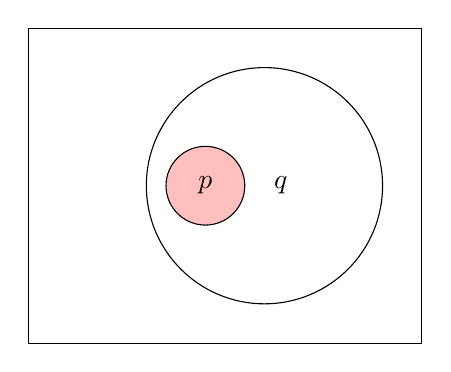
\begin{tikzpicture}
\filldraw[fill=white] (-2,-2) rectangle (3,2);
\scope % A \vee B
%\clip (0,0) circle (1);
\fill[pink] (0.25,0) circle (0.5);
%\fill[white] (0,0) circle (1);
\endscope
\draw (0.25,0) circle (0.5) node [text=black] {$p$}
      (1,0) circle (1.5) node [text=black,right] {$q$};
% outline
\end{tikzpicture}}
&
\scalebox{2}{
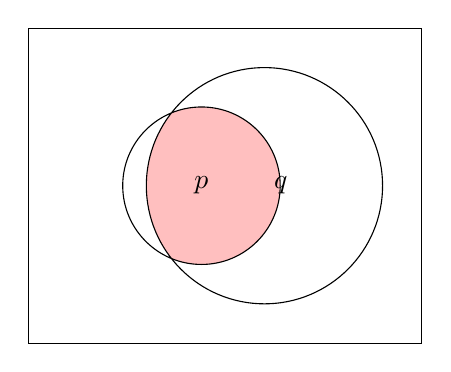
\begin{tikzpicture}
\filldraw[fill=white] (-2,-2) rectangle (3,2);
\scope % A \vee B
\clip (1,0) circle (1.5);
\fill[pink] (0.2,0) circle (1);
%\fill[white] (1,0) circle (1);
\endscope
\draw (0.2,0) circle (1) node [text=black] {$p$}
      (1,0) circle (1.5) node [text=black,right] {$q$};
% outline
\end{tikzpicture}}

\end{tabular}


\myslide{Generalized Quantifiers:  \iz{some}, \iz{no}} 
\begin{tabular}{cc}
some $p$ are $q$ & no $p$ are $q$ \\[2ex] 
\scalebox{2}{
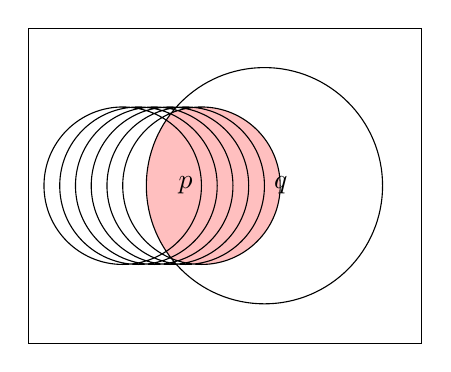
\begin{tikzpicture}
\filldraw[fill=white] (-2,-2) rectangle (3,2);
\scope % A \vee B
\clip (1,0) circle (1.5);
\fill[pink] (0.2,0) circle (1);
%\fill[white] (0,0) circle (1);
\endscope
\draw (-0.8,0) circle (1) 
      (-0.6,0) circle (1) 
      (-0.4,0) circle (1) 
      (-0.2,0) circle (1) 
      (0.0,0) circle (1) node [text=black] {$p$}
      (0.2,0) circle (1) 
%      (0.25,0) circle (0.5) 
      (1,0) circle (1.5) node [text=black,right] {$q$};
% outline
\end{tikzpicture}}
&
\scalebox{2}{
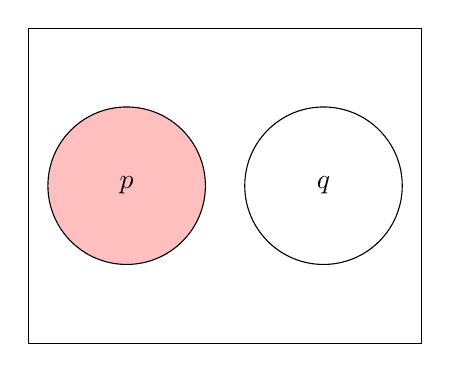
\begin{tikzpicture}
\filldraw[fill=white] (-2,-2) rectangle (3,2);
\scope % A \vee B
%\clip (1,0) circle (1.5);
\fill[pink] (-0.75,0) circle (1);
%\fill[white] (1,0) circle (1);
\endscope
\draw (-.75,0) circle (1) node [text=black] {$p$}
      (1.75,0) circle (1) node [text=black] {$q$};
% outline
\end{tikzpicture}}

\end{tabular}



\myslide{Strong/Weak Quantifiers}
\begin{exe}
  \ex only \txx{weak} quantifiers can occur in existential \eng{there} sentences
  \begin{xlist}
      \ex \eng{There is \ul{a} fox in the henhouse}
      \ex \eng{There are \ul{two} foxes in the henhouse}
      \ex \eng{*There is \ull{every} fox in the henhouse}
      \ex \eng{*There are \ull{both} foxes in the henhouse}
  \end{xlist}
\end{exe}
\begin{itemize}
\item \txx{symmetrical} (cardinal) quantifiers are \ul{\txx{weak}}
  \\ det(A,B) = det(B,A)
  \begin{exe}
    \ex \eng{three lecturers are Australian}   = \eng{three Australians are lecturers}
  \end{exe}
\item \txx{asymmetrical} (proportional) quantifiers are \ull{\txx{strong}}
  \\ det(A,B) $\ne$ det(B,A)
  \begin{exe}
    \ex \eng{most lecturers are Australian}   $\ne$ \eng{most Australians are lecturers}
  \end{exe}
\item[?] Come up with some more strong and weak quantifiers\task

\end{itemize}

\myslide{Negative Polarity Items (NPI)}
\begin{itemize}
\item Some words in English mainly appear in negative environments
  \begin{exe}
    \ex
    \begin{xlist}
      \ex \eng{Kim does\ull{n't} \ul{ever} eat dessert}
      \ex *\eng{Kim does \ul{ever} eat dessert}
    \end{xlist}
    \ex
    \begin{xlist}
      \ex \eng{Kim has\ull{n't} eaten dessert \ul{yet}}
      \ex *\eng{Kim has eaten dessert \ul{yet}}
    \end{xlist}
    \ex
    \begin{xlist}
      \ex \eng{Few people  have eaten dessert \ul{yet}}
      \ex *\eng{Many people have eaten dessert \ul{yet}}
    \end{xlist}
   \ex
    \begin{xlist}
      \ex \eng{Rarely does Kim \ul{ever} eat dessert}
      \ex *\eng{Often does Kim \ul{ever} eat dessert}
    \end{xlist}
  \end{exe}
\item Not just negation, but also some quantifiers
\item[?] Come up with some NPIs and environments\task
\end{itemize}

\myslide{Monotonicity}

\begin{itemize}
\item Some quantifiers control entailment between sets and subsets
  \begin{itemize}
  \item \txx{Upward entailment} goes from a subset to a set
  \item \txx{Downward entailment} goes from a set to a subset
  \end{itemize}
\end{itemize}

\begin{exe}
  \ex
  \begin{xlist}
    \ex \eng{Kim does\ull{n't} eat dessert} \ent  \eng{Kim does\ull{n't} eat hot dessert}
    \ex \eng{Kim does\ull{n't} eat hot dessert} \nent  \eng{Kim does\ull{n't} eat dessert}
    \trans \textbf{Downward entailment}
    \end{xlist}
    \ex
  \begin{xlist}
    \ex \eng{Kim eats some desserts} \nent  \eng{Kim eats hot desserts}
    \ex \eng{Kim eats some hot desserts} \ent  \eng{Kim  eats some desserts}
    \trans \textbf{Upward entailment}
    \end{xlist}
  \end{exe}
  \begin{itemize}
  \item \emp{Negative Polarity Items} are licensed by \emp{downward entailing expressions}
  \item Formal models of quantification can be used to make predictions
    about seemingly unrelated phenomena
\end{itemize}

\myslide{In other languages too!}

\MyLogo{Thanks to Joanna Sio and OpenAi}

\begin{exe}
\ex \glll {} \cmn{我} \cmn{没有} \cmn{任何} \cmn{朋友}  \\
        {} wo mei-you  renhe pengyou    \\
        {} I   \textsc{neg}-have any     friend \\
\trans ``I don't have any friends.''
\ex \glll * \cmn{我} \cmn{有} \cmn{任何} \cmn{朋友} \\
        {} wo you  renhe pengyou    \\
        {} I  have any     friend \\
\trans *''I have any friends.''
\end{exe}

\begin{exe}
\ex \gll {} \ces{Nemám} \ces{žádné} \ces{přátele.} \\
        {} \textsc{neg.have.1sg} any friends \\
\trans ``I don't have any friends.''
\ex \gll * \ces{Mám} \ces{žádné} \ces{přátele.} \\
        {} \textsc{have.1sg} any friends \\
\trans *``I have any friends.''
\end{exe}

\myslide{Negation Scope}

Negation can be triggered by many things, and the elements can be far away.

\begin{exe}
  \ex \eng{\ul{The German} was sent for but professed to \ul{know}
    \ull{nothing} \ul{of the matter} \ldots} (\sh{HOUN})
\ex \eng{I trust that \ul{there is} \ull{nothing} \ul{of consequence
which I have overlooked}?”}
\ex \eng{“A dabbler in science, Mr. Holmes, a picker up
of shells on the shores of \ul{the} great \ull{un}\ul{known
ocean}.}
\ex \eng{Our client looked down with a rueful face at \ul{his}
own \ull{un}\ul{conventional appearance}.}
\end{exe}
  



\section{Sentiment and Connotation}

\myslide{Connotation}
Many words carry more meaning than just identifying their referent.

\begin{exe}
  \ex
  \begin{xlist}
    \ex \eng{Kim is slender}
    \ex \eng{Kim is thin}
    \ex \eng{Kim is haggard}
  \end{xlist}
  \ex
  \begin{xlist}
    \ex \eng{The young lout is here.}
    \ex \eng{The young boy is here.}
    \ex \eng{The young gentleman is here.}
  \end{xlist}
  \ex
  \begin{xlist}
    \ex \eng{The young lout is arrogant.}
    \ex \eng{The young boy is proud.}
    \ex \eng{The young gentleman is confident.}
  \end{xlist}
 \ex
  \begin{xlist}
    \ex \eng{That bitch is cheap.}
    \ex \eng{That woman is economical.}
    \ex \eng{That lady is frugal.}
  \end{xlist}

\end{exe}

\myslide{Sentiment in the Holmes corpus}
\begin{itemize}
\item Doyle often gives us not-so subtle cues as to whether characters are
good or bad.
\item Some of them are very nationalist (and borderline racist, but not always)

\begin{exe}
  \ex \eng{A large face, seared with a thousand wrinkles, burned
    yellow with the sun, and marked with every \ul{evil} passion, was
    turned from one to the other of us, while his deep-set, \ul{bile}-shot
    eyes, and the high thin fleshless nose, gave him somewhat the
    resemblance to a fierce old bird of prey.} (\sh{SPEC})
  \ex \eng{He was a \ul{fine} creature, this \ul{man of the old English
    soil}, \ul{simple}, \ul{straight} and \ul{gentle}, with his
    \ul{great}, \ul{earnest}, \ul{blue eyes} and broad, \ul{comely face}. } (\sh{DANC})

  \ex \eng{``The aborigines of the Andaman Islands may perhaps claim
    the distinction of being the smallest race upon this earth, \ldots
    They are naturally \ul{hideous}, having large, \ul{misshapen} heads, small,
    fierce eyes, and \ul{distorted} features.''} (\sh{SIGN})
\item \eng{There was a portrait within of a man, \ul{strikingly
      handsome} and \ul{intelligent}, but bearing unmistakable signs
    upon his features of his African descent.} (\sh{YELL})

\end{exe}

\item[?] Can you find some examples of clearly positive or negative descriptions?\task
\end{itemize} 

\myslide{Sentiment and Composition}
\MyLogo{Sentiment Analysis/Opinion Mining is very popular these days}
\begin{itemize}
\item Sentiment can be built up.
  \begin{exe}
    \ex \eng{good} \hfill{$\uparrow$}
    \ex \eng{very good}  \hfill{$\uparrow\uparrow$}
    \ex \eng{less than very good}  \hfill{$\downarrow$}
    \ex \eng{I have never found it to be less than very good} \hfill{$u\uparrow\uparrow\uparrow$}
  \end{exe}
\item It can be complex
 \begin{exe}
   \ex \eng{The new story is good, especially the characterization,
     although the dialogue is a little stiff.}
  \end{exe}
 \item Polarity can depend on the target
 \begin{exe}
   \ex \eng{The screen is very wide.}
   \ex \eng{Their nostrils are very wide.}
  \end{exe}
\item It can come from other things than lexical cues: $\star\star\star\star\star$
%★★★★★ 
\end{itemize}

\myslide{Annotating Sentiment}
\MyLogo{Sentiment Analysis/Opinion Mining is very popular these days}
   \begin{tabular}{r>{\itshape}l>{\itshape}l>{\itshape}l>{\itshape}l}
      \textbf{Score} & \textbf{Example} & \textbf{Example} & \textbf{Example} & 
      \textbf{Corpus Examples} \\
      \hline
      95 & fantastic & very good     &            & {perfect}, splendidly  \\ 
      64 & good      & good          &            & {soothing}, pleasure  \\
      34 & ok        & sort of good  & not bad    & {easy}, interesting  \\ 
      0  & beige     & neutral       &            & {puff}  \\  
      -34 & poorly    & a bit bad     &            & rumour, cripple  \\
      -64 & bad       & bad           & not good   & {hideous}, death  \\
      -95 & awful     & very bad      &            & {deadly}, horror-stricken     
   \end{tabular}

   We annotate \txx{senses}: words given their meaning, before they
   are transformed by the syntax.  So \lex{good} in \eng{That is very
     very good}
   and \lex{good} in \eng{That is no good} get the same score.
   
% \end{itemize}



\begin{itemize}
\item Note that most words carry no sentiment.
\end{itemize}



 
 \myslide{High and Low Examples in multiple languages}
\newcommand{\ili}[1]{\href{https://lr.soh.ntu.edu.sg/omw/omw/concepts/ili/#1}{\url{i#1}}}

\begin{center}
\begin{small}
  \begin{tabular}{lrr>{\itshape}lrlrlr}
    Concept & freq & score & English & score & Chinese & score & Japanese & Score \\
    \hline
    % 01036996-n
    \ili{40833}  &   24 &  50 & marriage & 39 & 婚事 & 34 & 結婚	& 58\\
            &      &  & wedding  & 34 \\   
            % 02021905-a
    \ili{11080}  & 5& 40  &  rich & 33 & 有钱 & 34 &  裕福 & 66  \\
    % 06878071-n
    \ili{72643} & 4 & 33 &  smile &   32 & 微笑	& 34 & 笑み & 34 \\
    % 00358431-v
    \ili{23529}  & 40 & $-$68  & die & $-$80 &  去世 & $-$60 &亡くなる & $-$63 \\
            &        &  &  &       & 死亡  & $-$64 & 死ぬ & $-$62\\
            % 00220522-n
    \ili{36562}  & 5  & $-$83 & murder &$-$95  & 谋杀 & $-$95	 & 殺し & 	$-$64 \\
            &     &      && & & & 殺害 & $-$63 \\
  \end{tabular}
\end{small}
  
\end{center}

By generalizing to the concept, we can share sentiment values across
languages \citep{Bond:Ohkuma:daCosta:Miura:Chen:Kuribayashi:Wang:2016,Bond:Janz:Piasecki:2019}.


\section{Presupposition}

\myslide{Presuppositions}

\begin{itemize}
\item Many statements assume the truth of something else
  \begin{exe}
    \ex   \begin{xlist}
    \ex \eng{Mary's sister bakes the best pies.} %(presupposing sentence p)
    \ex \eng{Mary has a sister.} %(presupposition q)
    \end{xlist}
  \end{exe}
\item Negating the presupposing sentence $a$ doesn't affect the presupposition $b$
\item Names presuppose that their referents exist
\item Triggers 
  \begin{itemize}
  \item Clefts (\eng{it was X that Y}); Time adverbial; Comparative
  \item Factive verbs: \eng{realize}; 
    some judgement verbs: \eng{blame}; 
    some change of state: \eng{stop}
    \end{itemize}
\end{itemize}



% \myslide{Presuppositions}
%   To presuppose something means to assume it

% He’s stopped handing in his homework on time.
% b)  He used to hand in his homework on time.
% a) 

% Semantics or pragmatics?
% Truth relations
% 2)  Communications act
% 1) 

\myslide{Semantic approach}

\begin{itemize}
\item
  \begin{tabular}[t]{cll}
    $p$ & \eng{Mary's sister bakes the best pies}  & presupposing sentence\\
    $q$ & \eng{Mary has a sister}  & presupposition
  \end{tabular}
\begin{center}
    \begin{tabular}{|c|c|c|}
    \cline{1-3}
    $p$ &  & $q$   \\
    \cline{1-3}
    T & $\rightarrow$  & T  \\ 
    F & $\rightarrow$  & T \\ 
    F, T & $\leftarrow$  & T  \\ 
%    T & $\leftarrow$  & T  \\ 
    \cline{1-3}
  \end{tabular}
\end{center}
\item Also true of:
  \begin{tabular}[t]{cll}
   $\neg p$ & \eng{Mary's sister doesn't bake the best pies}
 \end{tabular}

\item Is that different from this? \\[2ex]
  \begin{tabular}{ll}
$a$ & \eng{I gave my dog a bath today.} \\
$b$ & \eng{I gave an animal a bath today.}
  \end{tabular}
\end{itemize}

\myslide{Presupposition versus entailment}
\begin{itemize}
\item  Negating the presupposing sentence does not affect the
presupposition whereas negating an entailing sentence
destroys the entailment.
\item  Can you think of other examples that show this difference?
\end{itemize}

\myslide{Interactional approach}
\begin{itemize}
\item  Presupposition is one aspect of a speaker's strategy of
organizing information for maximum clarity for the listener.
\begin{exe}
  \ex  \eng{Mary's sister bakes the best pies.} 
  \textnormal{
  \begin{xlist}
    \ex  Assertion 1: \eng{Mary has a sister X.}
    \ex  Assertion 2: \eng{X bakes the best pies.}
  \end{xlist}}
\end{exe}
\item  Assertion 1 is in the \txx{background} (old information)
\item  Assertion 2 is in the \txx{foreground} (new information)
\end{itemize}
   
\myslide{Presupposition failure}
\begin{itemize}
\item 
  \begin{exe}
  \ex  \eng{The King of France is bald.}
  \ex  \eng{There is a King of France.} \hfill presupposition
\end{exe}
\item  The problem with names and definite description is that they
presuppose the existence of the named or described entities.
\item  Solution: A speaker's use of a name or
definite description to refer usually carries a guarantee that the
listener can identify the referent.
\end{itemize}

\myslide{Presupposition triggers}
\begin{itemize}
\item  \txx{Cleft construction}
\begin{exe}
\ex  \eng{It was his nonsense that irritated me.}
\ex  \eng{What irritated me was his nonsense.} (pseudo)
\ex  \eng{Something irritated me.} \hfill presupposition
\end{exe}
\item  \txx{Time adverbial}
\begin{exe}
\ex  \eng{I was working five jobs before you went to school}
\ex  \eng{You went to school.} \hfill presupposition
\end{exe}
\item  \txx{Comparative}
\begin{exe}
\ex  \eng{You are even more silly than he is.}
\ex  \eng{He is silly.} \hfill presupposition
\end{exe}
\end{itemize}

\myslide{Presupposition triggers: Lexical triggers}
\begin{itemize}
\item  \txx{Factive verbs} presuppose the truth of their complement clauses.
  \begin{exe}
    \ex \begin{xlist}
      \ex  \eng{The students realized that Alex was hungry.}
      \ex  \eng{The students thought that Alex was hungry.} \hfill no presupposition
    \end{xlist}
    \ex \begin{xlist}
      \ex  \eng{Alex regretted not eating lunch.}
      \ex  \eng{Alex considered not eating lunch.} \hfill no presupposition
    \end{xlist}
  \end{exe}
\item  \txx{Verbs of judgement}
  \begin{exe}
    \ex \eng{Kim blamed me for making a mistake}
  \end{exe}
\item \txx{Change of state} (sometimes)
    \begin{exe}
      \ex \eng{Alex stopped talking to their imaginary friend.}
      \ex \eng{Have you stopped beating your dog?}
    \end{exe}
\end{itemize}

\myslide{Presupposition and context}
\begin{itemize}
\item  Presuppositions are context dependent. 
\begin{exe}
    \ex \begin{xlist}
      \ex \eng{John ate before going to the movies.}
      \ex  \eng{John went to the movies.} \hfill presupposition
    \end{xlist}
 \ex \begin{xlist}
   \ex $^{??}$\eng{John died before going to the movies}
   \ex  \eng{John went to the movies.} \hfill presupposition
 \end{xlist}
\end{exe}
\item Presuppositions are \txx{defeasible}: they can be canceled
  given the right context.
% due to the context of knowledge
% is known as defeasibility.

\end{itemize}


\myslide{Conclusions}

\begin{itemize}
\item Language can be used to reason
\item We reason unconsciously when we decide which words to use
\item Language can be used to convey impressions and opinions
  \begin{itemize}
  \item You will try to measure this as part of projects 1 and 2
  \end{itemize}
\item \citet{Saeed:2015} talks about Logic and Truth in Chapter~4
\item  \citet{Kroeger:2022} talks about Truth and Inference in Chapter~3 (meaning relations, presupposition), and the Logic of Truth in Chaper~4 (propositional logic, quantifiers).  He goes into more detail in Chapters~13, Modeling Compositionality, and~14 Quantifiers  
\end{itemize}


\small
\bibliographystyle{aclnat}
\bibliography{abb,mtg,nlp,ling}

\myslide{Glossary of Key Terms (English--Czech)}

\begin{longtable}{ll}
  English & Česky \\\hline \endhead
argument & argument \\
asymmetrical & asymetrický \\
background & pozadí \\
change of state & změna stavu \\
cleft construction & klivní konstrukce \\
comparative & komparativ \\
compositional Semantics & kompoziční sémantika \\
conclusion & závěr \\
deductive reasoning & deduktivní usuzování \\
defeasible & porazitelný / zvratitelný \\
denotational semantic analysis & denotační sémantická analýza \\
disjunctive syllogism & disjunktivní sylogismus \\
downward entailment & dolní implikace \\
empirical & empirický \\
entailment & implikace / logický závěr \\
equivocation & dvojsmysl / záměna významů \\
existential quantifier & existenciální kvantifikátor \\
factive verbs & faktivní slovesa \\
false dilemma & falešné dilema \\
foreground & popředí \\
guilt by association & vina sdružením / vina z asociace \\
hypothetical syllogism & hypotetický sylogismus \\
if & jestliže \\
iff & právě tehdy, když \\
individual constants & individuální konstanty \\
inductive Reasoning & induktivní usuzování \\
interpretation & interpretace \\
material implication & materiální implikace \\
not & ne \\
no true Scotsman & žádný pravý Skot (klam) \\
or & nebo \\
predicates & predikáty \\
premise & premisa \\
senses & významy \\
slippery slope & kluzký svah (klam) \\
strong & silný \\
symmetrical & symetrický \\
time adverbial & příslovečné určení času \\
truth conditions & pravdivostní podmínky \\
truth values & pravdivostní hodnoty \\
universal quantifier & univerzální kvantifikátor \\
upward entailment & horní implikace \\
variables & proměnné \\
verbs of judgement & slovesa úsudku \\
weak & slabý \\
xor & exkluzivní nebo / buď anebo \\
\end{longtable}

% \myslide{The Argument Clinic} 

% \begin{itemize}
% \item A sketch from episode 29 of
%   Monty Python's Flying Circus
% \item \textit{An argument is a connected series of statements intended to establish a proposition}
% \end{itemize}





\end{document}

%%% Local Variables: 
%%% coding: utf-8
%%% mode: latex
%%% TeX-PDF-mode: t
%%% TeX-engine: xetex
%%% End: 

